\documentclass[12pt]{article}
\usepackage{array}
\usepackage{amsmath}
\usepackage{amssymb}
\usepackage{algorithm}
\usepackage{algorithmic}
\usepackage{caption}
\usepackage{fontspec}
\usepackage{graphicx}
\usepackage{indentfirst}
\usepackage{minted}
\usepackage{mathtools}
\usepackage{pifont}
\usepackage{setspace}
\usepackage{subfigure}
\usepackage{tikz}
\usepackage{url}
\usepackage{xcolor}
\usepackage{xeCJK}

\usepackage[colorlinks=true]{hyperref}
\usepackage[margin=0.55in]{geometry}

% background color for minted
\definecolor{bg}{rgb}{0.95,0.95,0.95}

% CJK font
\setCJKmainfont{Source Han Serif CN}

% indent value
\setlength{\parindent}{2em}

% line spacing
\linespread{1.2}

% C++ styled text
\newcommand{\CC}{C\nolinebreak\hspace{-.05em}\raisebox{.4ex}{\tiny\bf +}%
\nolinebreak\hspace{-.10em}\raisebox{.4ex}{\tiny\bf +}}

\renewcommand{\thesection}{\Roman{section}}
\renewcommand{\thesubsection}{\thesection-\arabic{subsection}}

\title{简记Ray Tracing in One Weekend}
\author{Yiteng Zhang}

\begin{document}
\maketitle

\noindent{}\textbf{注:}Peter Shirley的\textit{Ray Tracing in One Weekend}系列对入门学习来说是特别友好的,在写下这篇
简记的时间点,这个系列已经非常有名了。之前有幸读过比较早期的1.X版本,最近听闻该系列的小书推出了一个较大的更新版本,
不免十分好奇,想要了解一下新版本的内容变更。另一方面,确实也想再回顾一下这本有趣的小书,所以又一次找出来
读一读(写这篇简记时,版本为3.2.3)。总体来看,新版本是有较多变化的,不但修正了旧版本的一些有误之处,也开始使用
一些modern {\CC}\,特性对之前的实现进行重构(尽管作者想尽量避免使用新特性)。无论如何,这本书是值得多次阅读的。
回到主题,这篇简记并非作为其翻译(也不太想那样做),实际上已经有不少这样的工作,做得相当好,译文很容易获得。
本文应该也不会大量说明具体的实现细节,因为书中详细地给出了所有的代码,没有任何模糊之处,而且在这里再贴一遍代码也
不会对行文与陈述有特别的好处。想来简记的作用也只能是尽量从书中的文字和代码片段中提炼出一些要点,避免以后每次回看
都频繁陷入实现细节之中,方便更好地把握书中所涉及的原理和技术的脉络。

\medskip
\indent{}显然,\textit{Ray Tracing in One Weekend}这本书是讲渲染的。具体来说,是讲述有关如何从零开始构建
一个光线追踪渲染器(即Raytracer)的书。此书不打算讨论渲染领域中涉及到的艰深部分,而是以体验式的方
式,手把手地带领我们领略光线追踪渲染的美妙所在。尽管不打算实现一个功能完备的渲染器,其讲述方式却也并不随便,反而可以说是
比较严谨的,不会让人感觉学不到真东西。

\indent{}想要渲染图像,那我们最后肯定是要得到能够真真切切看得到的结果。常见的图像格式都有自己的编解码过程,想要
不借助第三方库而得到对应的图像格式还是比较困难的。当然了,一些比较常用的header-only库如\texttt{stb\_image}可以帮我们
做这件事,但毕竟还是有一些额外工作要做。针对这个问题,书中推荐使用PPM格式,简单查一下就可以发现它是直接存文本的,只要能
找到合适的PPM解析器,就可以直接看到渲染出来的图像了,可以让我们暂时不必考虑出图编码的问题。

\indent{}渲染基础涉及到的数学知识基本上就是一点儿线性代数的内容,所以首先需要写代码来处理向量并实现一些辅助函数,大体上
是点积、叉积、向量单位化,还有求向量长度这些基本操作。具体的实现书里给出了一个,我们也可以自己写。无论如何,实现
这些操作总归是挺简单的事情,真正需要考虑的要点是约定这些操作函数的输入输出形式,以方便后续使用。

\indent{}一旦完成了上面的准备工作,就可以开始考虑如何绘制我们的三维场景。第一个问题是,ray是怎样的东西?
Ray tracing意为光线追踪,而这里的ray实际上也是符合射线(ray)的几何定义的。我们从一个端点$\bf{A}$出发,沿着某个方向
$\bf{b}$发出一条射线(或者说光线),其描述应该是:
\begin{equation}
\label{equ:ray}
\mathbf{P}(t) = \mathbf{A} + t\mathbf{b},\; t\in\mathbb{R}
\end{equation}
\noindent{}注意到$t$可以是负的,也就是说沿着与方向$\bf{b}$相反的方向投射。

\indent{}我们清楚光线追踪的核心原理:从相机中心朝着screen上的每个像素发出ray,这些ray与场景中的物体相交,通过计算
交点处的颜色来得到对应像素的颜色。现在我们已经清楚ray的表达,是时候对相机进行建模了,来看一个简单的例子:
\begin{figure}[h]
\centering
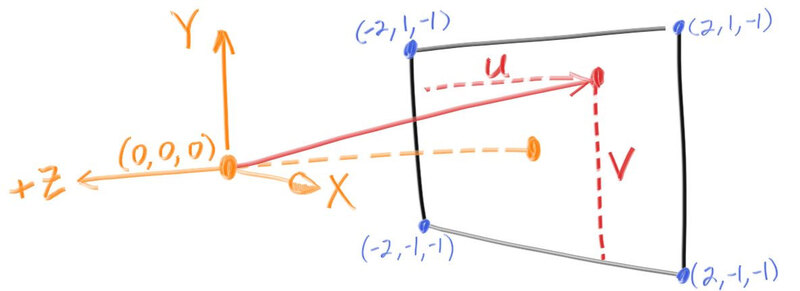
\includegraphics[width=0.6\textwidth]{./imgs/fig-1.03-cam-geom.jpg}
\end{figure}

\indent{}可以看到该相机直接被放在世界坐标系的原点,因而对应的相机坐标系的原点与世界坐标系的原点是重合的。另外,该相机的三个轴也
是与世界坐标系的坐标轴align的,可以说是相当特殊而又简单的一个例子,这便于我们进行渲染器的初期构建。同时,注意到相机中心到
投影平面的距离被设置为单位距离,这也是一项简化,可以说我们的virtual camera的焦距是单位值。
另一个细节是,为了更好区分垂直和水平方向(这有利于检查程序行为是否正常),可以使用非$1:1$宽高比(aspect ratio)的图像
尺寸比例,而相机视口的宽高比可取与图像宽高比相同的值以保持标准的正方像素间距。

\indent{}现在我们可以轻松写出从相机中心射向screen上任意位置的射线的表达式,因为可以根据上述相机模型给出式~\ref{equ:ray}~所需的
出射点$\mathbf{A}$和方向$\mathbf{b}$,即相机中心和它到screen上某一位置的方向向量。现在我们的世界中除相机外
空无一物,像素的颜色如何确定呢?可以想象,我们可能会看到一片蓝天,书中也给出了一种用于绘制简单蓝天效果的方法。
该方法的主要思想是,根据光线方向向量在垂直方向上的分量,对白色$(1.0,1.0,1.0)$和蓝色$(0.5,0.7,1.0)$进行线性混合,
或者说进行线性插值。

\indent{}如果一切正常工作,上面的过程可以给出一张具有颜色渐变效果的蓝色背景。下面考虑做点更有趣的事情,向世界
中添加一些物体。对光线追踪而言,球体可以算得上是最简单的物体之一了,因为计算球体与射线的相交并不复杂。
回想一下,中心在$(C_x, C_y, C_z)$且半径为$r$的球体为:
\begin{equation}
\label{equ:sphere}
(x - C_x)^2 + (y - C_y)^2 + (z - C_z)^2 = r^2
\end{equation}
我们试着用向量化的描述让上式~\ref{equ:sphere}~看起来更优雅简洁一些(在图形学中总是倾向于这样做),记球体中心位置
$\mathbf{C} = (C_x, C_y, C_z)$,与球上一点$\mathbf{P} = (x,y,z)$,那么球的方程为:
\begin{equation}
\label{equ:spherev}
(\mathbf{P} - \mathbf{C}) \cdot (\mathbf{P} - \mathbf{C}) = r^2
\end{equation}
如果有射线$\mathbf{P}(t)$与球相交,那么一定有满足~\ref{equ:spherev}~的$t$存在,我们来找一找这样的$t$:
\begin{displaymath}
(\mathbf{P}(t) - \mathbf{C}) \cdot (\mathbf{P}(t) - \mathbf{C}) = r^2
\end{displaymath}
然后将其展开为:
\begin{equation}
\label{equ:raysecball}
t^2 \mathbf{b} \cdot \mathbf{b}
    + 2t \mathbf{b} \cdot (\mathbf{A}-\mathbf{C})
    + (\mathbf{A}-\mathbf{C}) \cdot (\mathbf{A}-\mathbf{C}) - r^2 = 0
\end{equation}
\noindent{}想知道射线是否与球相交,只需要检查~\ref{equ:raysecball}~是否有根即可,根的个数即交点个数。

\indent{}可以通过简单的步骤验证一下上面方法的是否管用。我们可以在相机正前方一定距离处放一个大小合适的球,如果光线可以
击中球(即与球相交),我们就让对应的像素为红色$(1.0,0,0)$,否则仍绘制天空背景。如果实现正确,应该可以看到图像正中有一个
红色的圆形区域。这个红色区域现在看起来只是一个二维圆形,没有体现球的三维形态,因为我们不过是简单地设置了颜色,而没有
做真正有意义的shading,也未考虑反射和场景中多个物体的相互影响等因素,这些都是重要内容。

\indent{}现在开始尝试简单的shading,做一下表面法线的颜色映射。球面的法线即为交点处垂直于球体表面向外的
向量(一般用单位向量),其方向是$\mathbf{P}-\mathbf{C}$的方向,不妨记法向量为$\mathbf{n}$($\mathbf{n}$是
单位向量)。法向量的颜色映射可以使用一种简单的技巧来做:由于分量$(n_x, n_y, n_z)$的值落在区间$[-1,1]$上,我们可以
使用$(\frac{1+n_x}{2},\frac{1+n_y}{2},\frac{1+n_z}{2})$将分量的值的范围映射到$[0,1]$上,并对应到RGB颜色。上述过程
需要计算法向量,像之前那样仅判断光线与物体是否相交是不够的,还需要知道确切的交点位置,但实际上只需算出最近的交点即可。
一元二次方程的求根公式可以帮我们做到这一点。

\indent{}现在我们的场景中只有一个球体,但一般来说场景不会这么简单。为了支持对包含多个不同对象的场景进行渲染,书中详细
地介绍了一种\texttt{Hittable}抽象类的定义和用途,为渲染器提供了这项功能支持,并将球体类实现为它的派生类。
作为一个通用的实现,书中提到了设计时的一项要点:法线方向与光线方向的关系。对球体来讲,如果像前述场景那样,
光线从球的外部射过来并且与球相交于球上某一点$\mathbf{P}$,那么法线方向$\mathbf{P}-\mathbf{C}$总是向外的。
但是,必须要考虑到光线由球内部向外射的情形,这种情况确实需要被纳入考虑,比如当我们想要处理一个玻璃球时。
\begin{figure}[h]
\centering
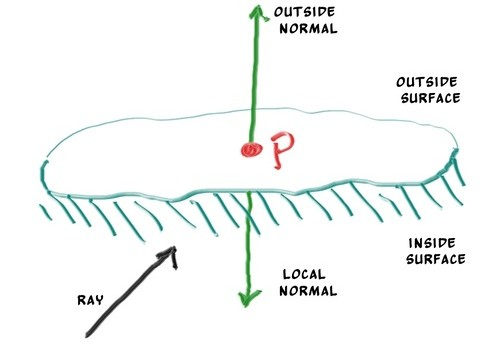
\includegraphics[width=0.45\textwidth]{./imgs/fig-1.06-normal-sides.jpg}
\end{figure}

\indent{}显然,当光线从球内部向外射时,法线方向应该是朝内的。在确定交点处法线方向时,可以用点积来判断,只需要
将光线的方向向量投影到方向朝外的法向上(即点积所作的事情),并检查投影方向与该方向是否相同即可(即检查点积
结果的正负),若不同则说明光线是从外部射过来的。

\indent{}做好这层抽象后,就可以通过维护一个\texttt{Hittable}对象的list来用同一套代码同时处理场景中的多个不同对象。
可以再向场景中添加一个很大的球作为地面,经过渲染后,我们得到的不再是之前的圆形红色区域,而是一个带有类似法线贴图
色彩效果的结果。

\indent{}现在我们的球看起来会有一些立体感,但效果并不好。另外,仔细观察会发现球的边缘呈现出锐利的锯齿状,很明显
这是因为没有使用抗锯齿(反走样)技术的缘故。在真实拍摄的图像中,边缘是没有这样的锯齿的,因为边缘处的像素混合了
一些背景和前景,我们也可以通过一些技术来达到相似的效果。书中介绍了一种抗锯齿方法,其思想是:不像之前那样
仅对每个像素做一次采样,而是在每个像素内进行多次采样并取它们的均值作为最终颜色。

\indent{}书中详细介绍了具体的实现方式。需要给出对应于采样分布是$[0,1)$上的均匀分布的随机数生成器\texttt{random},还可以
利用它给出$[V_{min},V_{max})$上的随机数生成器$V_{min} + (V_{max} - V_{min}) * \texttt{random()}$。函数\texttt{random}
的实现可以利用\texttt{<cstdlib>}的\texttt{rand}函数来做,也可以直接使用{\CC}\,的\texttt{<random>}中提供的均匀分布
随机数生成器来做,都是常用的方法。

\indent{}通过使用抗锯齿技术,渲染质量往往可以得到很大的提升。下图摘自原书中用于介绍抗锯齿技术的原理图,红色的框代表一个
pixel,黑色的点代表计算得到的像素内的随机位置。渲染时,为了计算该像素最终颜色,从相机中心向这几个黑点位置发出一束
射线,并射入场景中求交,然后将每条线对应的结果求平均作为与该像素对应的最终结果。
\begin{figure}[h]
\centering
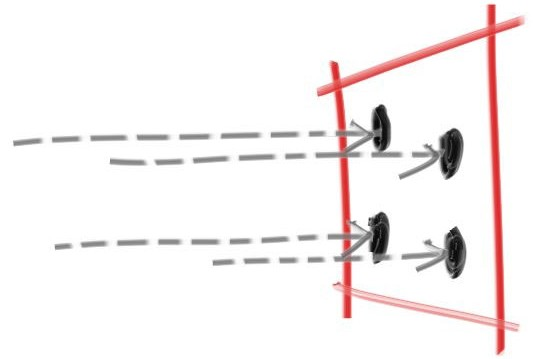
\includegraphics[width=0.4\textwidth]{./imgs/fig-1.07-pixel-samples.jpg}
\end{figure}

\indent{}到目前为止,一直是从比较偏几何的角度来考虑渲染过程。为了得到质量较好的渲染效果,场景对象的材质
属性是必须要考虑的因素,不同的材质属性决定了物体如何与光进行交互。光线射到物体上时如何反射,是否会有折射,
表面对光的吸收效果如何等等,有许多需要考虑的问题。

\indent{}一类常见的表面本身并不发射光线,而是将附近环境的颜色与其自身的固有颜色进行调制,且向外反射的光线方向是
随机的。光线“撞”在表面上时还会被吸收一部分能量,因而越是呈现出深暗颜色的表面,光被吸收得越多,看起来就比较黑。
具有此类特性的表面,光线与其交互的作用被认为是呈现出漫反射(diffuse reflection)。书中首先介绍了一种简单的
方法来实现这种效果,并说明该方法被用作一种“lazy hack”来近似理想漫反射。实际上,使用产生随机反射方向的任何算法
都能产生类似的哑光(matte)效果,而不一定必须是理想漫反射(被称为朗伯反射)。

\indent{}书中给出的这一“lazy hack”的方法是简单易行的。对于处于球面外侧,在“撞击点”与球面相切的单位球,其中心
位于$\mathbf{P}+\mathbf{n}$,其中$\mathbf{n}$为表面法线。我们要做的是在该单位球内(包括面上)随机地找
一点$\mathbf{S}$,则光与表面的相交点$\mathbf{P}$处的反射光线的方向沿$\mathbf{S}-\mathbf{P}$。
\begin{figure}[h]
\centering
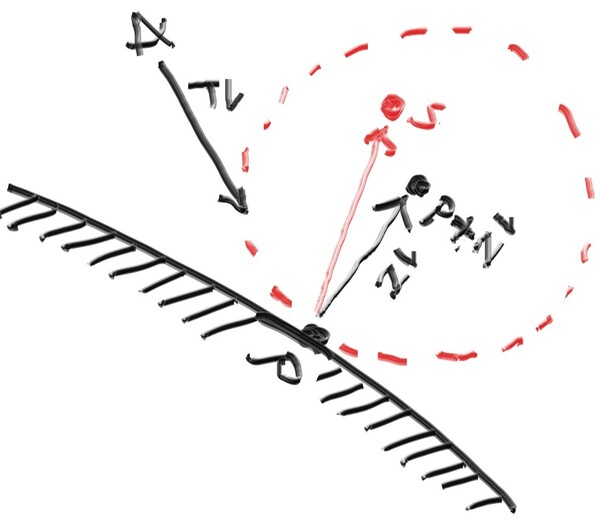
\includegraphics[width=0.42\textwidth]{./imgs/fig-1.09-rand-vec.jpg}
\end{figure}

\indent{}上述过程并不复杂,但关键的问题在于如何在单位球中随机选点。这种时候,拒绝采样(rejection sampling)总是简单
有效的。首先,我们在单位球的bounding box中采样,该box内的点的$x$,$y$与$z$上的取值均位于$[-1,1]$上(以球心为中心),
如果采样点落在单位球外,则拒绝。

\indent{}在书的目前版本中,明确说明上述方法是一种“lazy hack”。这并非是说这个方法不对,而是表明它并非准确的朗伯反射。
在比较早期的版本中,似乎直接将其作为理想漫反射进行展示,读者Vassillen Chizhov指出上述方法实际上给出的是$cos^{3}(\phi)$
分布($\phi$是偏离法向的角度),而非与真正的朗伯反射对应的$cos(\phi)$分布(可参考朗伯余弦定律)。
要做到真正的朗伯反射实际上并不会多费多少功夫,只需要将“在单位球内选点”更改为“在单位球上选点”即可,把前者的结果
归一化一下就可以了。

\indent{}实现时的一个重要细节是,光线会在场景中不断地与物体相撞,然后反射,然后再相撞。光线在这一递归过程中可能不再与物体相交
(即来自天空的光经过数次反射进入眼中),也可能会经过非常多次反射之后还在不断地进行下去。由于光在每次反射时是会被吸收的,
并且从技术的角度来看,不可能让它任意多次地进行下去(计算量太大,栈空间亦有限),我们应该对执行深度进行限制,一旦超出限制,
我们直接终止这一过程,并认为对应像素的颜色足够黑。

\indent{}接下来考虑具有金属材质属性的表面是如何与光进行交互的。日常的经验告诉我们,金属表面是具有金属光泽的平滑表面。
对于这样的表面,反射光的方向不会有太大的随机性,而是表现出接近镜面反射的特性。对于理想的平整金属表面,可以认为
呈现镜面反射。
\begin{figure}[h]
\centering
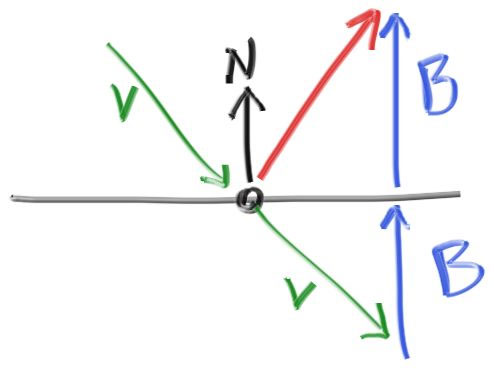
\includegraphics[width=0.4\textwidth]{./imgs/fig-1.11-reflection.jpg}
\end{figure}

\indent{}若令向量$\mathbf{v}$代表入射光(不一定是单位向量),则反射光可以用$\mathbf{v}+2\mathbf{b}$表示。
其中,向量$\mathbf{b}$的长度为$|\mathbf{v}\cdot\mathbf{n}|$,$\mathbf{n}$是法向量(是单位向量),则反射光
由$\mathbf{v}-(2\mathbf{v}\cdot\mathbf{n})\mathbf{n}$确定。

\indent{}如果我们向场景中添加以上述方式实现的金属球,会发现渲染结果与现实中看到的大多金属物体并不像,一个重要原因
是它现在太过光滑了,遵从理想的镜面反射。我们通常看到的金属表面并没有那么光滑,所以考虑实现一种带有磨砂
效果的金属表面。
\begin{figure}[h]
\centering
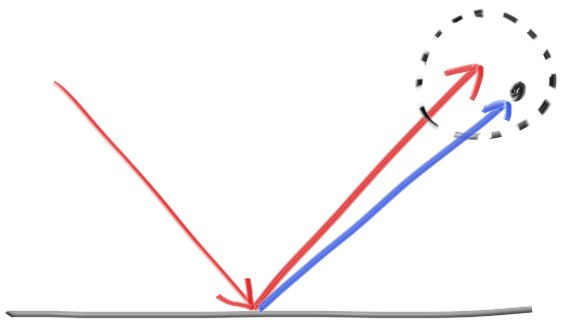
\includegraphics[width=0.45\textwidth]{./imgs/fig-1.12-reflect-fuzzy.jpg}
\end{figure}

\indent{}书中给出了一种为金属表面添加磨砂效果的方法,其思想相当易懂,只需要给反射光增加一点随机性即可。
如上图所示,在一个小的球内随机选择一点作为向量的新端点就可以了。显然,这个小球的半径影响磨砂效果,半径越小,
表面就越光滑。注意新的端点可能位于金属表面的内侧,这时我们可以认为光被完全吸收了,这可以通过使用点积检查出射光方向是否与
法向同侧进行确定。

\indent{}书中介绍的第三类材质是透明的介电质(dielectrics),比如水、玻璃和钻石等等。
介电质材质与光交互的一大特点是会有折射(refraction)发生,但同时又有反射发生。
在实现时,每次与光线交互时可以随机选择反射或折射进行计算,只处理其中一种即可。
\begin{figure}[h]
\centering
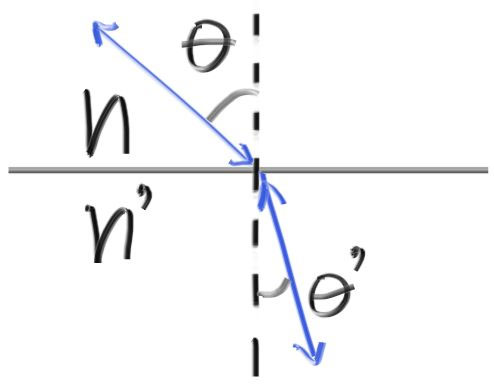
\includegraphics[width=0.4\textwidth]{./imgs/fig-1.13-refraction.jpg}
\end{figure}

\indent{}折射现象在物理上可由斯涅尔定律 (Snell's law)进行描述,该定律也是我们实现透明介电质渲染的主要依据。
斯涅尔定律说明:
\begin{equation}
\label{equ:snell}
\eta \cdot \sin\theta = \eta' \cdot \sin\theta'
\end{equation}

\indent{}具体来说,若有入射光$\mathbf{R}$以与入射点处的法线$\mathbf{n}$成夹角$\theta$的方向,从折射率为$\eta$的一侧射向
折射率为$\eta'$的一侧,则折射光$\mathbf{R}'$的方向与另一侧法线$\mathbf{n}'$间的夹角为$\theta'$。它们之间的关系
由~\ref{equ:snell}~确定。

\indent{}可以看到,两侧介电质折射率之间的比率可以刻画折射光的偏折程度。折射率(refractive index)是材质的
属性,描述了光在介电质中能跑多快。我们可以通过设置介电质的折射率来描述特定的介电质材质。比如真空的折射率是1.0,
而玻璃的折射率在1.3$\sim$1.7范围,这是书中主要讨论的材质。

\indent{}在实现时,入射光$\mathbf{R}$是已知的,我们关注的是如何得到折射光$\mathbf{R}'$的表达。根据向量分解,折射光
可被分解在水平方向上和垂直方向上(相对于法向$\mathbf{n}'$),描述为:
\begin{equation}
\mathbf{R'} = \mathbf{R'}_{\bot} + \mathbf{R'}_{\parallel}
\end{equation}
结合公式~\ref{equ:snell}~就可以得到:
\begin{align*}
&\mathbf{R'}_{\bot} = \frac{\eta}{\eta'} (\mathbf{R} + \cos\theta \mathbf{n})\\
&\mathbf{R'}_{\parallel} = -\sqrt{1 - |\mathbf{R'}_{\bot}|^2} \mathbf{n}
\end{align*}
若$\mathbf{R}$与$\mathbf{n}$都是单位向量,它们的点积即可确定$\cos\theta$,那么:
\begin{equation}
\mathbf{R'}_{\bot} = \frac{\eta}{\eta'} (\mathbf{R} + (\mathbf{-R} \cdot \mathbf{n}) \mathbf{n})
\end{equation}
则可据此计算$\mathbf{R'}_{\parallel}$,进而得到$\mathbf{R}'$关于$\mathbf{R}$的表达。

\indent{}通过上述过程,我们可以实现折射,但还有一个重要问题需要考虑。假设我们讨论的对象是玻璃球,那么
入射光从空气射入,经过一次折射后处于玻璃球内部,这个折射光还要继续传播,并再次撞到玻璃球表面上。这里
十分关键的一点是,玻璃的折射率大于空气,从玻璃内部射向其表面的光线可能并不会折射,因为可能发生的是
全内反射(total internal reflection)。

\indent{}具体来说,假如我们的玻璃球具有折射率$\eta=1.5$,而空气的折射率为$\eta'=1.0$(近似看作真空的折射率),
根据斯涅尔定律,空气一侧的折射光与法线夹角为:
\begin{equation}
\theta' = \sin^{-1}\bigg(\frac{\eta}{\eta'}\sin\theta\bigg)
\end{equation}
处于玻璃内部一侧的入射光与法线的夹角$\theta$大到一定程度,就没有$\theta'$的实解了。这种情况说明全内反射发生,
入射光全部向内面反射。在实现时要对该情况进行检查,判断应该处理折射还是反射。

\indent{}至此,我们的渲染器应该能给出效果还行的玻璃球渲染结果。书中不但规规矩矩地按照上述基础的物理规则进行
了实现,还提到了实践中常用的Fresnel-Schlick近似,也很值得进一步了解。

\indent{}将目前涉及的三种材质与场景中不同物体进行搭配,已经可以得到一些不错的渲染结果,但还有一项
重要的功能要考虑。对于场景渲染而言,相机也是场景中的一个物体而已,我们还希望能够从不同位置,使用不同的相机位姿来拍摄。
因此,还需要支持设定相机的朝向和姿态。这一部分的内容虽然十分基础,但也相当重要,在这里快速回顾一下。
\begin{figure}[h]
\centering
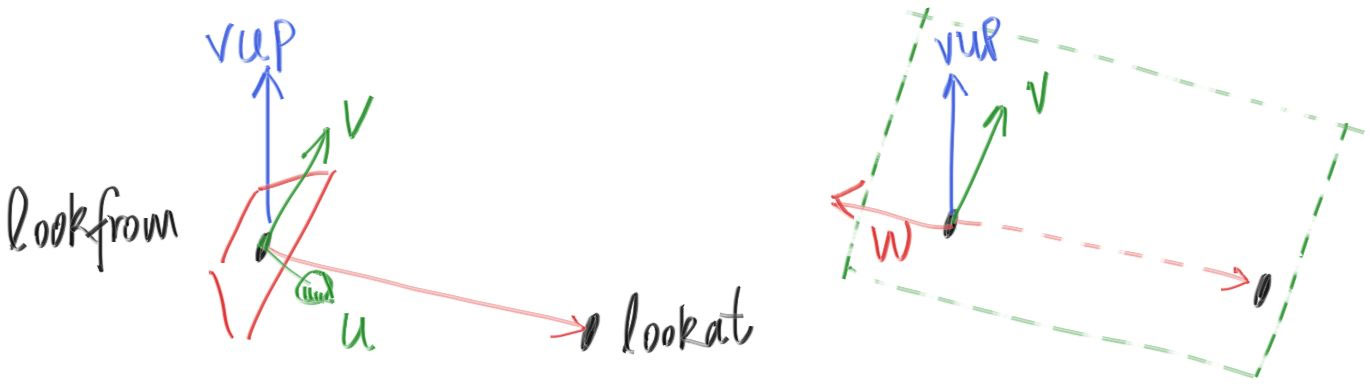
\includegraphics[width=0.8\textwidth]{./imgs/fig-1.16-cam-view-up.jpg}
\end{figure}

\indent{}对于调整相机位姿这件事情,可以试着想象我们正在使用相机来拍摄场景。
一方面,我们将相机放在某一位置,让它朝着另一个位置拍摄。另一方面,我们可以歪着相机来拍摄场景。
这两方面对相机的调整其实是分离的。具体来说,首先我们需要设定相机从哪里看,看向哪里。
我们将相机(其实是相机中心)放在世界中的某个位置lookfrom(定义在世界坐标系下),并给出另一个位置
lookat(定义在世界坐标系下),从lookfrom到lookat的方向就确定了相机朝向。与此同时,如果我们以这个方向
为轴旋转相机,就可以歪着拍摄。一般通过指定一个“vup”向量来描述相机的转动情况。比如,我们令向量vup为
$(0,1,0)$,则表示我们水平握持相机。

\indent{}这两方面都处理好后,就可以用一组正交基$(\mathbf{u}, \mathbf{v}, \mathbf{w})$来描述相机姿态,这对应于
相机坐标系的三个轴上的单位向量在世界坐标系下的表达。
lookfrom-lookat给出的方向可以直接确定$\mathbf{w}$的值。另外两个向量可以分别通过一次叉积得到,可用$\mathbf{vup}\times\mathbf{w}$
得到$\mathbf{u}$的值,再用$\mathbf{w}\times\mathbf{u}$得到$\mathbf{v}$的值,需要注意三个向量$\mathbf{u}$、$\mathbf{v}$和
$\mathbf{w}$都是单位向量,计算时需要做单位化。

\indent{}现在我们的渲染器具备了一些主要功能,并可渲染具有三类不同材质的球体。最后,书中拓展了景深(depth of field)这一增强性的功能,
用于使渲染结果看起来更加真实。可以想象,如果我们通过一个大的洞来成像,所有的东西都会是糊的,但如果我们
在这个洞里塞一个镜头,那么在某一个距离范围内的场景可以“对上焦”,成像是清晰的。目前我们并未遇到图像模糊的情况,毕竟
我们在使用理想的针孔模型,不会考虑失焦模糊。物理相机需要一个较大的洞来收集光,洞大进光量就多,这在摄影上对应于
光圈(aperture),我们前面构建的虚拟相机并未考虑这些影响因素,但真实相机确实需要一个放在洞里的透镜。
对于真实相机,如果需要更多的进光,就要使用大光圈,但这样洞也就大,会造成更多失焦。真实相机需要通过调整
镜头和传感器的相对距离使特定对象成像清晰。
虚拟相机不需要考虑进光量多少的问题,我们只需模拟光圈(即洞的大小)来实现失焦模糊的效果。

\indent{}在实现时,我们并不需要去模拟真实相机内部的一切,那是特别复杂而不必要的。书中使用了薄透镜模拟
(thin lens approximation),并让光从透镜上的某位置朝着focus plane发出,该平面到镜头的距离是一个可以设定的参数,
用于决定完全不失焦的距离。薄透镜意味着我们忽略镜头厚度,光线的出发点是一个圆盘上的随机位置,该圆盘以
lookfrom点为圆心。圆盘半径越大,失焦越明显。可以认为在我们之前的实现中这个半径是零,因而不发生任何失焦。

\indent{}最后,书中将前述所有核心内容综合在一起来构建场景,这里也展示一个渲染结果。我们以一个大球为地面,
首先在上面放置三个排成一列的球,分别表现为朗伯、玻璃和磨砂金属。然后,在地面上随机放一些大小相同的很小
的球,并随机为它们安排三种材质之一。最后加上景深效果,使近距离和远距离的场景失焦模糊。
\begin{figure}[h]
\centering
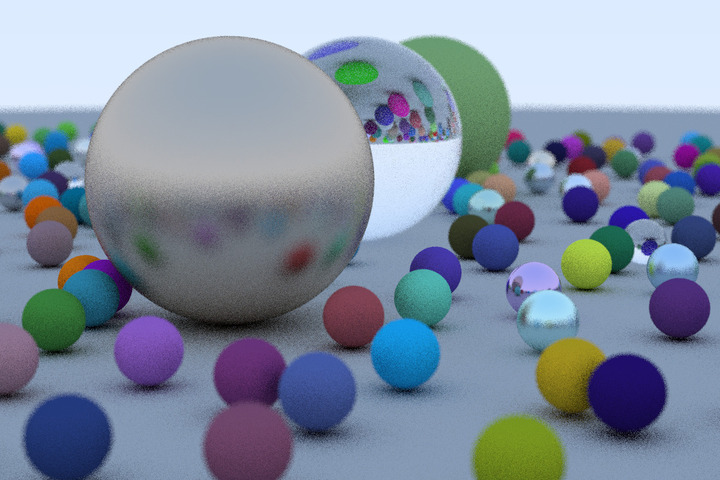
\includegraphics[width=\textwidth]{./imgs/balls.jpg}
\end{figure}

\end{document}